% Proposed replacement for Reviewer 1, Comment A2. This is an additive draft;
% it does not edit the active manuscript or response letter automatically.

\subsection*{A2. Train/test overlap for FT-600K}

\noindent\textbf{Reviewer comment.}
\begin{quote}
\itshape
``Rule out train/test overlap for FT-600K: report the minimum SOAP-distance (or RMSD) between each in-gap NEB image and its nearest fine-tuning frame, or re-run FT-600K with the NEB-adjacent trajectory segment excluded, and confirm the 0.16 eV result survives.''
\end{quote}

\noindent\textbf{Response.}
We agree that the relevant issue is not only literal frame duplication, but also whether the migration task is genuinely distinct from the configurations used for fine-tuning. The declared FT-600K fine-tuning corpus contains 600~K AIMD source trajectories only: no NEB image, NEB optimizer history, or NEB-adjacent trajectory segment was included as a fine-tuning frame. Consequently, an NEB-segment-exclusion retraining is not applicable; the target paths were excluded at the source-data level. We nevertheless added a direct geometry audit and changed the split from the former frame-wise shuffle to a trajectory-grouped split, assigning each complete AIMD source trajectory to exactly one partition (1,786/311/267 train/validation/test frames).

For the direct audit, we compared each of the 25 retained DFT fixed-path images from pathways 1--2, 1--3, 1--4, 1--5, and 1--7 with the declared grouped fine-tuning files. The full grouped training set contains zero exact global fingerprint matches, zero exact Cr-local fingerprint matches, zero images with Cr-centred SOAP cosine distance $\leq 10^{-4}$, and zero species-compatible local environments with RMSD $\leq 0.05$~\AA. Its closest SOAP neighbour is $5.43\times10^{-4}$ and its closest comparable Cr-local RMSD neighbour is 2.06~\AA. The 89-frame Scratch-5\% subset likewise gives zero SOAP-near and zero RMSD-near matches, with minima $6.37\times10^{-4}$ and 2.06~\AA, respectively. The RMSD calculation is intentionally reported only for species-composition-compatible Cr-local environments (two comparable candidates in the full grouped set and one in Scratch-5\%); it is not inflated into a claim about all non-comparable environments. These results rule out direct target-image leakage under the declared fingerprint, SOAP, and local-RMSD criteria. They do not make a claim about unknown foundation-model pretraining corpora, and SOAP proximity alone is not treated as leakage without an exact or low-RMSD correspondence (Fig.~\ref{fig:a2-distance-audits}; Table~\ref{tab:a2-direct-overlap}).

To make the broader task-distribution question explicit, we additionally show the available common SOAP/PCA diagnostic (Fig.~\ref{fig:a2-task-map}). In its retained historical reference fit, 250 AIMD training, 246 held-out AIMD, and 25 fixed-path NEB configurations occupy different projected regions. This map is descriptive rather than a calibrated uncertainty or leakage score, and it is not substituted for the direct grouped audit above. A separate 639-frame, stage-balanced large-cell MD failure-attribution sample lies outside the historical training kNN q99 envelope at every sampled stage. Importantly, its median kNN distance does not increase monotonically from early stable (12.69) through pre-onset (12.54) and precursor (12.21) to threshold (11.17). We therefore do not claim that a scalar descriptor distance causes instability or orders every task by difficulty. Instead, the combined evidence motivates the task-conditioned framework: held-out AIMD, fixed-path migration, and model-driven failure branches probe different directions of configuration space and require different validation operators.

Under the grouped re-evaluation, the historical frame-level 0.16~eV point estimate is not reproduced. On pathway~1--4, the absolute fixed-path barrier error relative to the provisional 0.34~eV DFT candidate is $0.47\pm0.12$~eV for three OMAT-FT-start FT-600K models, $1.20\pm0.27$~eV for Scratch, and $0.68\pm0.20$~eV for Scratch-5\%; the MPA0 comparator is a single-seed result (0.24~eV) and is not included in a seed-uncertainty estimate. We now retain 0.16~eV only as a historical frame-level reference and do not assert that it survives the leakage-controlled protocol.

\noindent\textbf{Manuscript changes.}
We will add the source-level NEB exclusion and the grouped direct-overlap audit to Methods Sec.~2.1, insert Table~\ref{tab:a2-direct-overlap} and Fig.~\ref{fig:a2-distance-audits} in the SI section ``Data splitting and configuration-space audit'', and cite the descriptive task map from the evaluation-framework discussion. The task map is currently SI-ready because its common reference fit is historical rather than the current grouped FT-600K train file. It becomes main-text-ready after a post-processing-only refresh with the archived grouped train/validation/test structures and the same descriptor transform; no new MD, NEB, or DFT calculation is required for that refresh. Self-relaxed NEB is kept outside this map until its model-relaxed images are transformed with that same grouped-training reference, because fixed-path and self-relaxed NEB are different measurement operators.

% Proposed SI table
\begin{table}[t]
\centering
\caption{\textbf{Direct A2 overlap audit for the 25 retained DFT fixed-path images.} The target images were compared with the declared trajectory-grouped fine-tuning files. A near match requires SOAP cosine distance $\leq 10^{-4}$ or, for a species-composition-compatible Cr-centred local environment, RMSD $\leq 0.05$~\AA. The absence of a near match establishes no detected direct target-image leakage under the declared metrics; it does not characterize an unknown foundation pretraining corpus.}
\label{tab:a2-direct-overlap}
\begin{tabular}{lccccc}
\toprule
Training split & Frames & Exact matches & Min. SOAP & Min. comparable RMSD & Near matches \\
\midrule
Full grouped & 1,786 & 0 global; 0 local & $5.43\times10^{-4}$ & 2.06~\AA & 0 SOAP; 0 RMSD \\
Scratch-5\% grouped & 89 & 0 global; 0 local & $6.37\times10^{-4}$ & 2.06~\AA & 0 SOAP; 0 RMSD \\
\bottomrule
\end{tabular}
\end{table}

% Proposed SI figure: direct response to reviewer A2.
\begin{figure}[t]
\centering
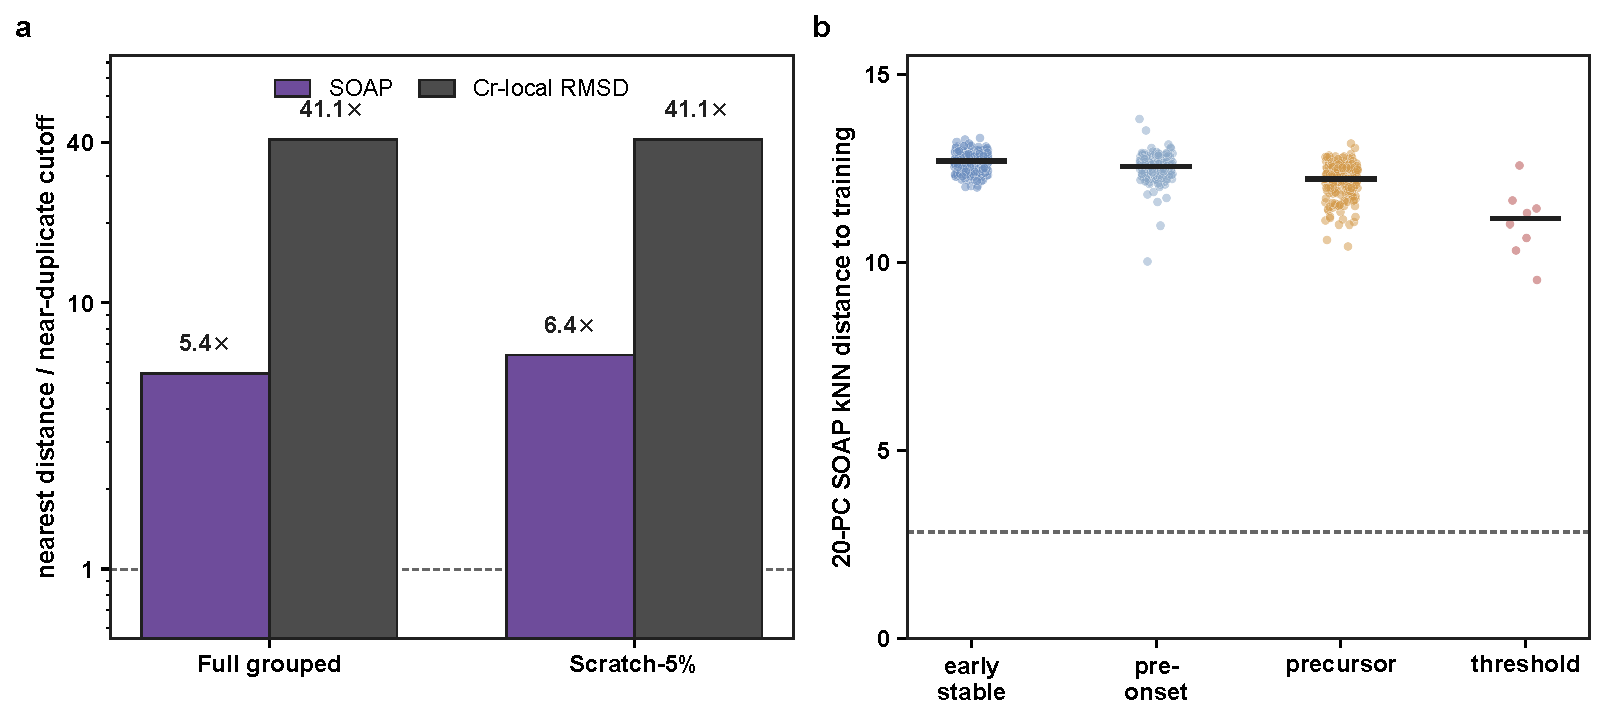
\includegraphics[width=\linewidth]{../response_to_reviewers/reviewer_a2_distribution_shift_task_ladder_20261018/figures/fig_a2_distance_audits.pdf}
\caption{\textbf{Direct leakage audit and a descriptor-space counterexample to a scalar difficulty ladder.} \textbf{a}, The closest target-image neighbour in each declared grouped training split is farther than the prespecified near-duplicate cutoff under both Cr-centred SOAP and comparable local RMSD; values are plotted as distance divided by the corresponding cutoff. \textbf{b}, In the separate historical 639-frame large-cell failure-attribution sample, all stage-balanced samples are outside the training kNN q99 envelope (dashed line), but their descriptor distances do not increase monotonically towards the instability threshold. Points are individual sampled frames and horizontal bars are medians. Panel~b is descriptive and does not establish a causal instability mechanism.}
\label{fig:a2-distance-audits}
\end{figure}

% Proposed SI figure; move to the main-text evaluation framework only after a
% common map is regenerated from the actual grouped FT-600K raw structures.
\begin{figure}[t]
\centering
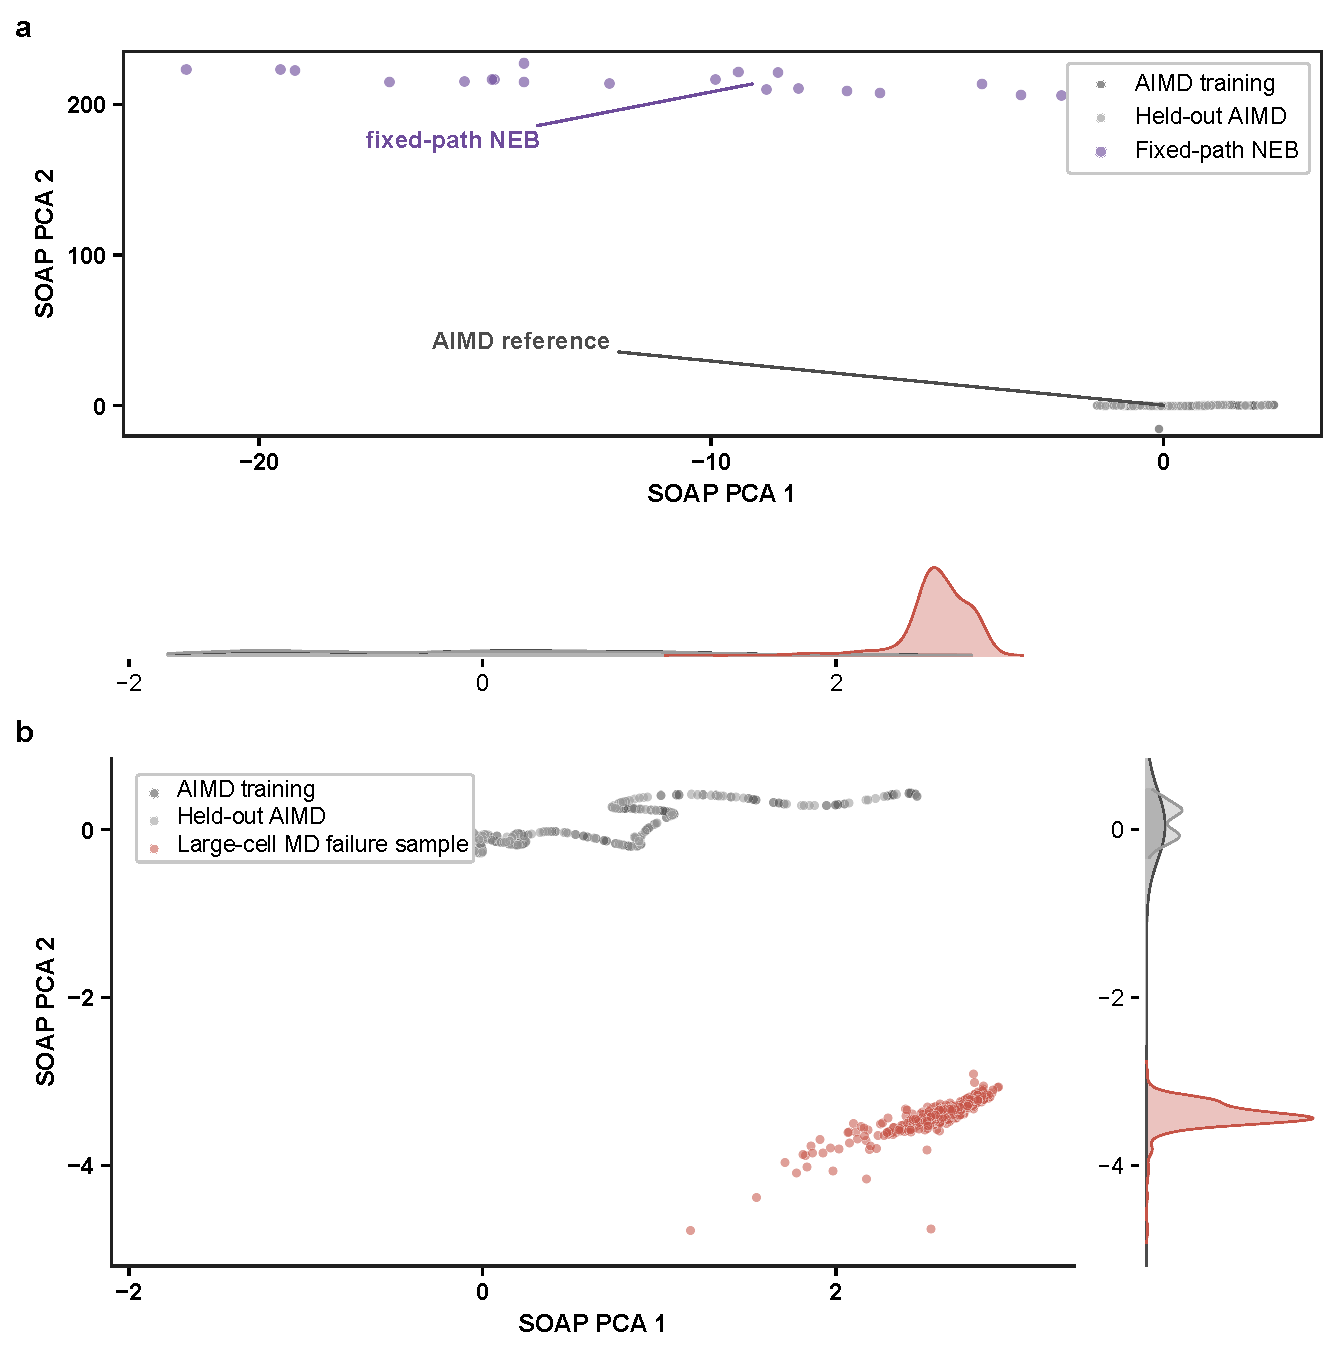
\includegraphics[width=\linewidth]{../response_to_reviewers/reviewer_a2_distribution_shift_task_ladder_20261018/figures/fig_a2_task_distribution_map.pdf}
\caption{\textbf{Descriptive task map in the retained historical SOAP/PCA reference fit.} \textbf{a}, The historical reference contains 250 AIMD training configurations, 246 held-out AIMD configurations, and 25 fixed-path NEB images. The fixed-path images occupy a distinct direction in the displayed projection. \textbf{b}, A detail view with matched marginal kernel-density estimates shows that the 639-frame, stage-balanced large-cell MD failure-attribution sample occupies another projected region. Coordinates are a visualization of the retained 20-component SOAP/PCA diagnostic; two-dimensional separation is not used as a calibrated OOD distance, a leakage test, or a model ranking.}
\label{fig:a2-task-map}
\end{figure}

% Proposed main-text insertion, after the grouped-split paragraph in Methods Sec. 2.1.
The fine-tuning files were constructed from 600~K AIMD source trajectories and contain no NEB images or NEB-optimizer history. To test for possible structural homology beyond this source-level exclusion, we compared each retained DFT fixed-path image with the declared grouped training file using exact global and Cr-local fingerprints, Cr-centred SOAP cosine distance, and species-compatible Cr-local RMSD. No exact or near-duplicate target image was detected under the declared criteria (Table~S\textnormal{[A2]}). We treat this audit as evidence against direct leakage, not as an assertion that a low-dimensional descriptor coordinate completely orders downstream task difficulty.

% Proposed evaluation-framework discussion insertion.
Configuration shift in MigrationBench is multidirectional rather than a single scalar radius from the training distribution. The available descriptive SOAP/PCA map separates held-out AIMD, fixed-path migration images, and a large-cell MD failure-attribution sample in different projected directions (Fig.~S\textnormal{[A2]}). The failure sample also shows that descriptor distance need not increase monotonically immediately before instability. These diagnostics therefore motivate task-specific stress tests; they do not substitute for DFT validation of a barrier or self-relaxed pathway.
